% Options for packages loaded elsewhere
\PassOptionsToPackage{unicode}{hyperref}
\PassOptionsToPackage{hyphens}{url}
%
\documentclass[
]{book}
\usepackage{amsmath,amssymb}
\usepackage{lmodern}
\usepackage{ifxetex,ifluatex}
\ifnum 0\ifxetex 1\fi\ifluatex 1\fi=0 % if pdftex
  \usepackage[T1]{fontenc}
  \usepackage[utf8]{inputenc}
  \usepackage{textcomp} % provide euro and other symbols
\else % if luatex or xetex
  \usepackage{unicode-math}
  \defaultfontfeatures{Scale=MatchLowercase}
  \defaultfontfeatures[\rmfamily]{Ligatures=TeX,Scale=1}
\fi
% Use upquote if available, for straight quotes in verbatim environments
\IfFileExists{upquote.sty}{\usepackage{upquote}}{}
\IfFileExists{microtype.sty}{% use microtype if available
  \usepackage[]{microtype}
  \UseMicrotypeSet[protrusion]{basicmath} % disable protrusion for tt fonts
}{}
\makeatletter
\@ifundefined{KOMAClassName}{% if non-KOMA class
  \IfFileExists{parskip.sty}{%
    \usepackage{parskip}
  }{% else
    \setlength{\parindent}{0pt}
    \setlength{\parskip}{6pt plus 2pt minus 1pt}}
}{% if KOMA class
  \KOMAoptions{parskip=half}}
\makeatother
\usepackage{xcolor}
\IfFileExists{xurl.sty}{\usepackage{xurl}}{} % add URL line breaks if available
\IfFileExists{bookmark.sty}{\usepackage{bookmark}}{\usepackage{hyperref}}
\hypersetup{
  pdftitle={Cellxgene VIP},
  pdfauthor={Kejie Li, Zhengyu Ouyang, Dongdong Lin, Michael Mingueneau, Will Chen, David Sexton, Baohong Zhang},
  hidelinks,
  pdfcreator={LaTeX via pandoc}}
\urlstyle{same} % disable monospaced font for URLs
\usepackage{color}
\usepackage{fancyvrb}
\newcommand{\VerbBar}{|}
\newcommand{\VERB}{\Verb[commandchars=\\\{\}]}
\DefineVerbatimEnvironment{Highlighting}{Verbatim}{commandchars=\\\{\}}
% Add ',fontsize=\small' for more characters per line
\usepackage{framed}
\definecolor{shadecolor}{RGB}{248,248,248}
\newenvironment{Shaded}{\begin{snugshade}}{\end{snugshade}}
\newcommand{\AlertTok}[1]{\textcolor[rgb]{0.94,0.16,0.16}{#1}}
\newcommand{\AnnotationTok}[1]{\textcolor[rgb]{0.56,0.35,0.01}{\textbf{\textit{#1}}}}
\newcommand{\AttributeTok}[1]{\textcolor[rgb]{0.77,0.63,0.00}{#1}}
\newcommand{\BaseNTok}[1]{\textcolor[rgb]{0.00,0.00,0.81}{#1}}
\newcommand{\BuiltInTok}[1]{#1}
\newcommand{\CharTok}[1]{\textcolor[rgb]{0.31,0.60,0.02}{#1}}
\newcommand{\CommentTok}[1]{\textcolor[rgb]{0.56,0.35,0.01}{\textit{#1}}}
\newcommand{\CommentVarTok}[1]{\textcolor[rgb]{0.56,0.35,0.01}{\textbf{\textit{#1}}}}
\newcommand{\ConstantTok}[1]{\textcolor[rgb]{0.00,0.00,0.00}{#1}}
\newcommand{\ControlFlowTok}[1]{\textcolor[rgb]{0.13,0.29,0.53}{\textbf{#1}}}
\newcommand{\DataTypeTok}[1]{\textcolor[rgb]{0.13,0.29,0.53}{#1}}
\newcommand{\DecValTok}[1]{\textcolor[rgb]{0.00,0.00,0.81}{#1}}
\newcommand{\DocumentationTok}[1]{\textcolor[rgb]{0.56,0.35,0.01}{\textbf{\textit{#1}}}}
\newcommand{\ErrorTok}[1]{\textcolor[rgb]{0.64,0.00,0.00}{\textbf{#1}}}
\newcommand{\ExtensionTok}[1]{#1}
\newcommand{\FloatTok}[1]{\textcolor[rgb]{0.00,0.00,0.81}{#1}}
\newcommand{\FunctionTok}[1]{\textcolor[rgb]{0.00,0.00,0.00}{#1}}
\newcommand{\ImportTok}[1]{#1}
\newcommand{\InformationTok}[1]{\textcolor[rgb]{0.56,0.35,0.01}{\textbf{\textit{#1}}}}
\newcommand{\KeywordTok}[1]{\textcolor[rgb]{0.13,0.29,0.53}{\textbf{#1}}}
\newcommand{\NormalTok}[1]{#1}
\newcommand{\OperatorTok}[1]{\textcolor[rgb]{0.81,0.36,0.00}{\textbf{#1}}}
\newcommand{\OtherTok}[1]{\textcolor[rgb]{0.56,0.35,0.01}{#1}}
\newcommand{\PreprocessorTok}[1]{\textcolor[rgb]{0.56,0.35,0.01}{\textit{#1}}}
\newcommand{\RegionMarkerTok}[1]{#1}
\newcommand{\SpecialCharTok}[1]{\textcolor[rgb]{0.00,0.00,0.00}{#1}}
\newcommand{\SpecialStringTok}[1]{\textcolor[rgb]{0.31,0.60,0.02}{#1}}
\newcommand{\StringTok}[1]{\textcolor[rgb]{0.31,0.60,0.02}{#1}}
\newcommand{\VariableTok}[1]{\textcolor[rgb]{0.00,0.00,0.00}{#1}}
\newcommand{\VerbatimStringTok}[1]{\textcolor[rgb]{0.31,0.60,0.02}{#1}}
\newcommand{\WarningTok}[1]{\textcolor[rgb]{0.56,0.35,0.01}{\textbf{\textit{#1}}}}
\usepackage{longtable,booktabs,array}
\usepackage{calc} % for calculating minipage widths
% Correct order of tables after \paragraph or \subparagraph
\usepackage{etoolbox}
\makeatletter
\patchcmd\longtable{\par}{\if@noskipsec\mbox{}\fi\par}{}{}
\makeatother
% Allow footnotes in longtable head/foot
\IfFileExists{footnotehyper.sty}{\usepackage{footnotehyper}}{\usepackage{footnote}}
\makesavenoteenv{longtable}
\usepackage{graphicx}
\makeatletter
\def\maxwidth{\ifdim\Gin@nat@width>\linewidth\linewidth\else\Gin@nat@width\fi}
\def\maxheight{\ifdim\Gin@nat@height>\textheight\textheight\else\Gin@nat@height\fi}
\makeatother
% Scale images if necessary, so that they will not overflow the page
% margins by default, and it is still possible to overwrite the defaults
% using explicit options in \includegraphics[width, height, ...]{}
\setkeys{Gin}{width=\maxwidth,height=\maxheight,keepaspectratio}
% Set default figure placement to htbp
\makeatletter
\def\fps@figure{htbp}
\makeatother
\setlength{\emergencystretch}{3em} % prevent overfull lines
\providecommand{\tightlist}{%
  \setlength{\itemsep}{0pt}\setlength{\parskip}{0pt}}
\setcounter{secnumdepth}{5}
\usepackage{booktabs}
\ifluatex
  \usepackage{selnolig}  % disable illegal ligatures
\fi
\usepackage[]{natbib}
\bibliographystyle{plainnat}

\title{Cellxgene VIP}
\author{Kejie Li, Zhengyu Ouyang, Dongdong Lin, Michael Mingueneau, Will Chen, David Sexton, Baohong Zhang}
\date{2021-09-29}

\begin{document}
\maketitle

{
\setcounter{tocdepth}{1}
\tableofcontents
}
\hypertarget{getting-started-with-cellxgene-vip}{%
\chapter{Getting started with cellxgene VIP}\label{getting-started-with-cellxgene-vip}}

This is a cellxgene VIP tutorial book written in \textbf{Markdown}.

\hypertarget{why-use-cellxgene-vip}{%
\section{Why use cellxgene VIP?}\label{why-use-cellxgene-vip}}

\hypertarget{getting-set-up}{%
\section{Getting Set up}\label{getting-set-up}}

\hypertarget{execute-anaconda}{%
\subsection{Execute anaconda}\label{execute-anaconda}}

\begin{Shaded}
\begin{Highlighting}[]
\NormalTok{bash }\SpecialCharTok{\textasciitilde{}}\ErrorTok{/}\NormalTok{Downloads}\SpecialCharTok{/}\NormalTok{Anaconda3}\FloatTok{{-}2020.02}\SpecialCharTok{{-}}\NormalTok{Linux}\SpecialCharTok{{-}}\NormalTok{x86\_64.sh}
\end{Highlighting}
\end{Shaded}

If anaconda is not installed on server, you can install it following anaconda documentation (\url{https://docs.anaconda.com/anaconda/install/linux/})
\#\#\# Create and enable conda environment

\begin{Shaded}
\begin{Highlighting}[]
\CommentTok{\# clone repo from cellxgene VIP github}
\NormalTok{git clone https}\SpecialCharTok{:}\ErrorTok{//}\NormalTok{github.com}\SpecialCharTok{/}\NormalTok{interactivereport}\SpecialCharTok{/}\NormalTok{cellxgene\_VIP.git}
\NormalTok{cd cellxgene\_VIP}

\CommentTok{\# conda environment}
\NormalTok{source }\SpecialCharTok{\textless{}}\NormalTok{path to Anaconda3}\SpecialCharTok{\textgreater{}}\ErrorTok{/}\NormalTok{etc}\SpecialCharTok{/}\NormalTok{profile.d}\SpecialCharTok{/}\FunctionTok{conda.sh}\NormalTok{ (Default}\SpecialCharTok{:} \ErrorTok{/}\NormalTok{opt}\SpecialCharTok{/}\NormalTok{anaconda3}\SpecialCharTok{/}\NormalTok{etc}\SpecialCharTok{/}\NormalTok{profile.d}\SpecialCharTok{/}\NormalTok{conda.sh)}
\NormalTok{conda config }\SpecialCharTok{{-}{-}}\NormalTok{set channel\_priority flexible}
\NormalTok{conda env create }\SpecialCharTok{{-}}\NormalTok{n }\SpecialCharTok{\textless{}}\NormalTok{env name, such as}\SpecialCharTok{:}\NormalTok{ VIP}\SpecialCharTok{\textgreater{}} \SpecialCharTok{{-}}\NormalTok{f }\FunctionTok{VIP.yml}\NormalTok{ (system}\SpecialCharTok{{-}}\NormalTok{wide R) or }\FunctionTok{VIP\_conda\_R.yml}\NormalTok{ (local R under conda, no root privilege needed)}
\NormalTok{conda activate }\SpecialCharTok{\textless{}}\NormalTok{env name, such as}\SpecialCharTok{:}\NormalTok{ VIP}\SpecialCharTok{\textgreater{}}
\NormalTok{or}
\NormalTok{source activate }\SpecialCharTok{\textless{}}\NormalTok{env name}\SpecialCharTok{\textgreater{}}
\end{Highlighting}
\end{Shaded}

\hypertarget{cellxgene-installation}{%
\subsection{Cellxgene installation}\label{cellxgene-installation}}

Install cellxgene by running config.sh in ``cellxgene\_VIP'' directory

\begin{Shaded}
\begin{Highlighting}[]
\NormalTok{.}\SpecialCharTok{/}\NormalTok{config.sh}
\end{Highlighting}
\end{Shaded}

\hypertarget{r-dependencies}{%
\subsection{R dependencies}\label{r-dependencies}}

Install all required R packages on linux:

\begin{Shaded}
\begin{Highlighting}[]
\NormalTok{export LIBARROW\_MINIMAL}\OtherTok{=}\NormalTok{false}
\CommentTok{\#  ensure that the right instance of R is used. e.g. system{-}wide: /bin/R or /usr/bin/R ; local R under conda: \textasciitilde{}/.conda/envs/VIP\_conda\_R/bin/R}
\NormalTok{which R}

\NormalTok{R }\SpecialCharTok{{-}}\NormalTok{q }\SpecialCharTok{{-}}\NormalTok{e }\StringTok{\textquotesingle{}if(!require(devtools)) install.packages("devtools",repos = "http://cran.us.r{-}project.org")\textquotesingle{}}
\NormalTok{R }\SpecialCharTok{{-}}\NormalTok{q }\SpecialCharTok{{-}}\NormalTok{e }\StringTok{\textquotesingle{}if(!require(Cairo)) devtools::install\_version("Cairo",version="1.5{-}12",repos = "http://cran.us.r{-}project.org")\textquotesingle{}}
\NormalTok{R }\SpecialCharTok{{-}}\NormalTok{q }\SpecialCharTok{{-}}\NormalTok{e }\StringTok{\textquotesingle{}if(!require(foreign)) devtools::install\_version("foreign",version="0.8{-}76",repos = "http://cran.us.r{-}project.org")\textquotesingle{}}
\NormalTok{R }\SpecialCharTok{{-}}\NormalTok{q }\SpecialCharTok{{-}}\NormalTok{e }\StringTok{\textquotesingle{}if(!require(ggpubr)) devtools::install\_version("ggpubr",version="0.3.0",repos = "http://cran.us.r{-}project.org")\textquotesingle{}}
\NormalTok{R }\SpecialCharTok{{-}}\NormalTok{q }\SpecialCharTok{{-}}\NormalTok{e }\StringTok{\textquotesingle{}if(!require(ggrastr)) devtools::install\_version("ggrastr",version="0.1.9",repos = "http://cran.us.r{-}project.org")\textquotesingle{}}
\NormalTok{R }\SpecialCharTok{{-}}\NormalTok{q }\SpecialCharTok{{-}}\NormalTok{e }\StringTok{\textquotesingle{}if(!require(arrow)) devtools::install\_version("arrow",version="2.0.0",repos = "http://cran.us.r{-}project.org")\textquotesingle{}}
\NormalTok{R }\SpecialCharTok{{-}}\NormalTok{q }\SpecialCharTok{{-}}\NormalTok{e }\StringTok{\textquotesingle{}if(!require(Seurat)) devtools::install\_version("Seurat",version="3.2.3",repos = "http://cran.us.r{-}project.org")\textquotesingle{}}
\NormalTok{R }\SpecialCharTok{{-}}\NormalTok{q }\SpecialCharTok{{-}}\NormalTok{e }\StringTok{\textquotesingle{}if(!require(rmarkdown)) devtools::install\_version("rmarkdown",version="2.5",repos = "http://cran.us.r{-}project.org")\textquotesingle{}}
\NormalTok{R }\SpecialCharTok{{-}}\NormalTok{q }\SpecialCharTok{{-}}\NormalTok{e }\StringTok{\textquotesingle{}if(!require(tidyverse)) devtools::install\_version("tidyverse",version="1.3.0",repos = "http://cran.us.r{-}project.org")\textquotesingle{}}
\NormalTok{R }\SpecialCharTok{{-}}\NormalTok{q }\SpecialCharTok{{-}}\NormalTok{e }\StringTok{\textquotesingle{}if(!require(viridis)) devtools::install\_version("viridis",version="0.5.1",repos = "http://cran.us.r{-}project.org")\textquotesingle{}}
\NormalTok{R }\SpecialCharTok{{-}}\NormalTok{q }\SpecialCharTok{{-}}\NormalTok{e }\StringTok{\textquotesingle{}if(!require(BiocManager)) devtools::install\_version("BiocManager",version="1.30.10",repos = "http://cran.us.r{-}project.org")\textquotesingle{}}
\NormalTok{R }\SpecialCharTok{{-}}\NormalTok{q }\SpecialCharTok{{-}}\NormalTok{e }\StringTok{\textquotesingle{}if(!require(fgsea)) BiocManager::install("fgsea")\textquotesingle{}}

\CommentTok{\# These should be already installed as dependencies of above packages}
\NormalTok{R }\SpecialCharTok{{-}}\NormalTok{q }\SpecialCharTok{{-}}\NormalTok{e }\StringTok{\textquotesingle{}if(!require(dbplyr)) devtools::install\_version("dbplyr",version="1.0.2",repos = "http://cran.us.r{-}project.org")\textquotesingle{}}
\NormalTok{R }\SpecialCharTok{{-}}\NormalTok{q }\SpecialCharTok{{-}}\NormalTok{e }\StringTok{\textquotesingle{}if(!require(RColorBrewer)) devtools::install\_version("RColorBrewer",version="1.1{-}2",repos = "http://cran.us.r{-}project.org")\textquotesingle{}}
\NormalTok{R }\SpecialCharTok{{-}}\NormalTok{q }\SpecialCharTok{{-}}\NormalTok{e }\StringTok{\textquotesingle{}if(!require(glue)) devtools::install\_version("glue",version="1.4.2",repos = "http://cran.us.r{-}project.org")\textquotesingle{}}
\NormalTok{R }\SpecialCharTok{{-}}\NormalTok{q }\SpecialCharTok{{-}}\NormalTok{e }\StringTok{\textquotesingle{}if(!require(gridExtra)) devtools::install\_version("gridExtra",version="2.3",repos = "http://cran.us.r{-}project.org")\textquotesingle{}}
\NormalTok{R }\SpecialCharTok{{-}}\NormalTok{q }\SpecialCharTok{{-}}\NormalTok{e }\StringTok{\textquotesingle{}if(!require(ggrepel)) devtools::install\_version("ggrepel",version="0.8.2",repos = "http://cran.us.r{-}project.org")\textquotesingle{}}
\NormalTok{R }\SpecialCharTok{{-}}\NormalTok{q }\SpecialCharTok{{-}}\NormalTok{e }\StringTok{\textquotesingle{}if(!require(MASS)) devtools::install\_version("MASS",version="7.3{-}51.6",repos = "http://cran.us.r{-}project.org")\textquotesingle{}}
\NormalTok{R }\SpecialCharTok{{-}}\NormalTok{q }\SpecialCharTok{{-}}\NormalTok{e }\StringTok{\textquotesingle{}if(!require(data.table)) devtools::install\_version("data.table",version="1.13.0",repos = "http://cran.us.r{-}project.org")\textquotesingle{}}
\end{Highlighting}
\end{Shaded}

\hypertarget{run-cellxgene-by-h5ad-file}{%
\subsection{Run cellxgene by h5ad file}\label{run-cellxgene-by-h5ad-file}}

You can aslo run cellxgene by specifying a h5ad file, which stores scRNA-seq data along with a host and a port.
Use `ps' to find used ports to spare. Please see \url{https://chanzuckerberg.github.io/cellxgene/posts/launch} for details

\begin{Shaded}
\begin{Highlighting}[]
\NormalTok{ps }\SpecialCharTok{{-}}\NormalTok{ef }\SpecialCharTok{|}\NormalTok{ grep cellxgene}
\NormalTok{Rscript }\SpecialCharTok{{-}}\NormalTok{e }\StringTok{\textquotesingle{}reticulate::py\_config()\textquotesingle{}}
\CommentTok{\# Run the following command if the output of the above command doesn\textquotesingle{}t point to the Python in your env.}
\NormalTok{export RETICULATE\_PYTHON}\OtherTok{=}\StringTok{\textasciigrave{}}\AttributeTok{which python}\StringTok{\textasciigrave{}}
\NormalTok{cellxgene launch }\SpecialCharTok{{-}{-}}\NormalTok{host }\SpecialCharTok{\textless{}}\NormalTok{xxx}\SpecialCharTok{\textgreater{}} \SpecialCharTok{{-}{-}}\NormalTok{port }\SpecialCharTok{\textless{}}\NormalTok{xxx}\SpecialCharTok{\textgreater{}} \SpecialCharTok{{-}{-}}\NormalTok{disable}\SpecialCharTok{{-}}\NormalTok{annotations }\SpecialCharTok{{-}{-}}\NormalTok{verbose }\SpecialCharTok{\textless{}}\NormalTok{h5ad file}\SpecialCharTok{\textgreater{}}
\end{Highlighting}
\end{Shaded}

\hypertarget{cellxgene-on-web-browser}{%
\subsection{Cellxgene on web browser}\label{cellxgene-on-web-browser}}

chrome is preferred, version 87.0.4280.88 or 87.0.4280.141 is used. Users can access \textbf{http(s)://host:port}.
Following screenshot is what you should be able to see in console of chrome developer tools.
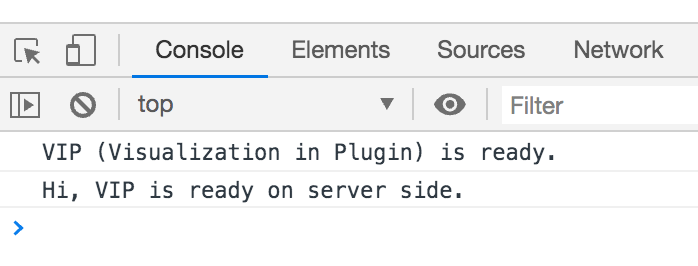
\includegraphics{cellonweb.png}

\hypertarget{install-instruction}{%
\chapter{Install instruction}\label{install-instruction}}

\hypertarget{install-anaconda-if-not-avaiable-on-server}{%
\section{Install anaconda if not avaiable on server}\label{install-anaconda-if-not-avaiable-on-server}}

All chapter sections start with a second-level (\texttt{\#\#}) or higher heading followed by your section title, like the sections above and below here. You can have as many as you want within a chapter.

\hypertarget{an-unnumbered-section}{%
\subsection*{An unnumbered section}\label{an-unnumbered-section}}
\addcontentsline{toc}{subsection}{An unnumbered section}

Chapters and sections are numbered by default. To un-number a heading, add a \texttt{\{.unnumbered\}} or the shorter \texttt{\{-\}} at the end of the heading, like in this section.

  \bibliography{book.bib,packages.bib}

\end{document}
